% !TEX root = ../thesis.tex

\section{Потокова модель задачі множення матриць}

Нехай система складається з $m$ обчислювальних вузлів та кожен з них характеризується швидкістю роботи $p_i , i=1,\ldots,m$ – тобто кількістю операцій з плаваючою точкою за секунду, які він може здійснити. Процесори з’єднані лініями зв’язку з планувальником, який передає задачі та приймає від них результат. Будемо вважати, що лінії зв’язку ідентичні та мають швидкість передачі даних $q$ та затримку $l$.
Будемо вважати, що виконуються наступні припущення
\begin{itemize}
	\item Всі процесори починають роботу одночасно
	\item Планувальник здійснює призначення миттєво
\end{itemize}

Нехай задані дві квадратні матриці розмірності $N \times N$ , результат множення яких необхідно обчислити. При використанні блочного алгоритму користувач задає розмір блоку $n$ , в результаті чого формуються $k=\frac{N^2}{n^2}$  задач, кожна з яких буде мати складність $\mathcal{O}(n^2)$ . Припустимо, що планувальник забезпечує пересилку повідомлень на вузли за певним фіксованим алгоритмом, який завершує обчислення за час $T(N,n)$. Тоді задача користувача полягає у пошуку мінімуму функції:

\begin{equation}
	\label{eq:general_minimization_problem}
	T(N,n) \longrightarrow \min
\end{equation}
\\
Функція $T(N,n)$ може мати багато локальних мінімумів в залежності від конфігурації системи. Ілюстрації графіків функції, отриманої шляхом симуляції, наведені у експериментальній частині та корелють з отриманими результатами у \cite{DoroshenkoIgnatenkoIvanenko}.

Одним з розповсюджених підходів до аналізу таких задач полягає у дослідженні потокової моделі даного процесу \cite{FluidModelForJobScheduling}.

Припустимо, що користувач вибрав вектор $x \in \mathbb{R}$ з компонентами $x_i$, де $x_i > 0$ , $x_i \le k$, $i=1,\ldots,m$, $\sum_{i=1}^{k}x_i = k$. Всі таки вектори утворюють множину $X(n)$ . Кожен компонент вектора $x$ описує відсоток задач, призначених для виконання на  $i$-тому процесорі. Будемо брати до уваги тільки операції, множення. Таке спрощення дозволяє у явному вигляді виписати функції часу. Загальний час закінчення залежить від  $x$, та дорівнює:

\begin{equation}
	\label{eq:total_time_general}
	T(x,X(n)) = \max\limits_{i=1,\ldots,m}{\frac{x_i N n^2}{p_i}}
\end{equation}
\\
Потокова модель передбачає можливість розділення задачі на підзадачі розміру $\epsilon = N n^2$, компонування з них підходящих підзадач та визначення загального часу при  $\epsilon \longrightarrow 0$.

Твердження 1.
Мінімальний час обчислень для потокової моделі з одним користувачем дорівнює:
\begin{equation}
	\label{eq:lema1}
	T = \frac{N^{3}}{\sum_{i=1}^{m}p_i}
\end{equation}
\\
Згізно з цим користувач має розділити задачі так, щоб вузол $i$ отримав задач з сумарною складністю $p_i*T$ часу.

Функція Мінковського для множини $X$ та вектора $p \in \mathbb{R}^m$ визначається наступним чином:

\begin{equation}
	\mu_X(p) = inf {\lambda > 0 : p \in \lambda X}
\end{equation}

Відомо, що ця функція опукла для опуклої $X$.
Визначимо множину потужностей системи $R = {r \in \mathbb{R}^m : r_i \in [0, p_i]}$ та масштабуємо її наступним чином:

\begin{equation}
	R(n) = \frac{R}{Nn^2}
\end{equation}

Тоді $ T(x, X(n)) = \mu_{R(n)}(x) $.
\\
Доведення.
\\
Розглянемо праву частину: $\mu_{R(n)}(x) = inf {\lambda > 0 : x \in \lambda R(n)}$ Умова належності вектора $x$ множині $R$ записується як $\max\limits_{i=1,\ldots,m} \frac{x_i Nn^2}{p_i}$,а значить $\mu_{X(n)}(p) = inf \big\{ \lambda > 0 : \max\limits_{i=1,\ldots,m} \frac{x_i}{p_i} = \frac{\lambda}{Nn^2} \big\}$. Або $\lambda = \max\limits_{i=1,\ldots,m} \frac{x_i Nn^2}{p_i}$. З властивостей функції $mu_{X(n)}(x)$ випливає, що мінімальний час $T_{min} = \min\limits_{x \in X(n)} $ існує і єдиний. Для врахування пересилок та затримки з'єднання потрібно зазначити, що алгоритм надсилає $2x_iNn$ елементів ( $x_i$ пар матриць розмірів $n*N$ ) на відповідний вузол $i$ та приймає $x_i*n^2$ елементів ( $x_i$ результатів множення матриць $n*N$ та $N*n$).

Отже, сумарний час закінчення з урахуванням пересилок та затримок дорівнює:
\begin{equation}
	\label{eq:main_time}
	T_s(x,X(n)) = \max\limits_{i=1,\ldots,m} \bigg\{ \frac{x_i N n^2}{p_i} + \frac{x_i (n^2 + 2 N n )}{q} + x_i l \bigg\}
\end{equation}

Твердження 2. Існує мінімум часу по $x - \min\limits_{x \in X(n)} T_s(x, X(n))$

\section{Аналіз штрафів від величини розбиття}

У цьому підрозділі ми проведемо аналіз того, як величина розбиття впливає на час виконання задач у потоковій моделі.

Як ми бачимо з \ref{eq:main_time}, наявні 2 види штрафів від дрібності розбиття. Перший вид з'являється через надлишковість передачі даних при розбитті матриці на підматриці, а другий напряму від кількості задач, що утворились в результаті розбиття.

Пронормуємо $x_i$:
\begin{equation}
	\label{eq:d_i}
	d_i = \frac{x_i}{\sum\limits_{i=1,\ldots,m} x_i} = \frac{x_i}{k}
\end{equation}

Таким чином $d_i$ це доля обчислень вузла $i$, $d_i \in [0, 1], \sum\limits_{i=1,\ldots,m} d_i = 1$. І навпаки, $x_i = d_i * k = d_i * \frac{N^2}{n^2}$

Перепишемо \ref{eq:main_time} за допомоги $d_i$:

\begin{equation}
	\label{eq:main_time_d_i}
	T_s(x,X(n)) = \max\limits_{i=1,\ldots,m} \bigg\{ \frac{d_i k N n^2}{p_i} + \frac{d_i k(n^2 + 2 N n )}{q} + d_i k l \bigg\}
\end{equation}

Проте нас більше всього цікавить рівняння із заміною $k = \frac{N^2}{n^2}$.

\begin{equation}
\label{eq:main_time_d_i_2}
T_s(x,X(n)) = \max\limits_{i=1,\ldots,m} \bigg\{ \frac{d_i \frac{N^2}{n^2} N n^2}{p_i} + \frac{d_i \frac{N^2}{n^2}(n^2 + 2 N n )}{q} + d_i \frac{N^2}{n^2} l \bigg\}
\end{equation}

Після скорочення отримаємо:

\begin{equation}
\label{eq:main_time_d_i_final}
T_s(x,X(n)) = \max\limits_{i=1,\ldots,m} \bigg\{ d_i \frac{N^3}{p_i} + d_i \frac{N^2 ( 1 + 2*\frac{N}{n} )}{q} + d_i \frac{N^2}{n^2} l \bigg\}
\end{equation}

Позначимо за $T_i$ час роботи вузла $i$, тоді:
\begin{equation}
	\begin{aligned} 
		T_i &= d_i \frac{N^3}{p_i} + d_i \frac{N^2 ( 1 + 2*\frac{N}{n} )}{q} + d_i \frac{N^2}{n^2} l \\
		T_s(x,X(n)) &= \max\limits_{i=1,\ldots,m} T_i
	\end{aligned} 
\end{equation}

Виділимо окремі складові $T_i$:
\begin{equation}
	\begin{aligned} 
		A_i &= \frac{N^3}{p_i} \\
		B_i &= \frac{N^2 ( 1 + 2*\frac{N}{n} )}{q} \\
		C_i &= \frac{N^2}{n^2} l \\
		T_i &= d_i ( A_i + B_i + C_i )
	\end{aligned} 
	\label{eq:T_i_parts}
\end{equation}

Таким чином ми розділили час виконання на 3 окремі складові, кожна з яких має свій сенс. Перша складова $A_i$ відповідає за сумарну складність алгоритма множення двох матриць без розбиття. Друга складова $B_i$ відповідає за надлишковість передачі даних і третя $C_i$ за затримки.

Причому помітимо, що $A_i$ ніяк не залежить від $n$. Тобто перша складова це завжди повна складність задачі множення цілих матриць і незалежно від розбиття складність блочного множення сумарно залишається незмінною.

Нехай фіксована конфігурація середовища, тобто $p_i, i=1,\ldots,m$ задані та незмінні. У такому випадку при зміні розбиття долі обчислень вважаємо незмінними, оскільки вони в першу чергу залежать від потужностей обчислювальних вузлів.

І для двох різних розбиттів $n_1$, $n_2$ : $n_1 < n_2$ ми маємо складові $A_i$ однаковими, оскільки вони не залежать від розбиття.

\begin{equation}
	\label{eq:diff_n1n2}
	\begin{aligned}
		& n_1, n_2 : n_1 < n_2
		\\
		&A_i^{n_1} = A_i^{n_2} = \frac{N^3}{p_i}
		\\
		&\frac{B_i^{n_1}}{B_i^{n_2}} = \frac{1 + 2*\frac{N}{n_1}}{1 + 2*\frac{N}{n_2}} =\frac{ n_2 ( n_1 + 2N ) }{n_1 ( n_2 + 2N )}
		\\
		&\frac{C_i^{n_1}}{C_i^{n_2}} = \bigg( \frac{n_2}{n_1} \bigg)^2
	\end{aligned}
\end{equation}

Візьмемо за $n_2=N$, оскільки як можна здогадатися, якщо ми матрицю не розрізаємо, тоді надлишковості немає. Тому будемо порівнювати випадок розрізання і множення цілої матриці на віддаленому вузлі. У такому випадку звісно з'являється проблема неефективного використання обчислювальної мережі, проте на даний момент нас цікавить дослідження надлишковості при множенні матриці блочно.

\begin{equation}
\label{eq:diff_n1n2}
	\begin{aligned}
	& n_1, n_2 : n_1 < n_2, n_2 = N
	\\
	& r_{n_1} = \frac{N}{n_{1}}
	\\
	& \frac{B_i^{n_1}}{B_i^{N}} =\frac{ N ( n_1 + 2N ) }{n_1 ( N + 2N )} = \frac{n_1 + 2N}{3n_1} = \frac{1 + 2r_{n_1}}{3}
	\\
	& \frac{C_i^{n_1}}{C_i^{n_2}} = \bigg( r_{n_1} \bigg)^2
	\end{aligned}
\end{equation}

Для наглядності побудуємо графік відношення $\frac{B_i^{n_1}}{B_i^{N}}$ для деяких віксованих N. Будемо брати $n_1 \in [50, N]$ щоб не мати проблем з маштабом оскільки при малих $n_1$ це відношення дуже велике.

\begin{figure}[H]
	\centering
	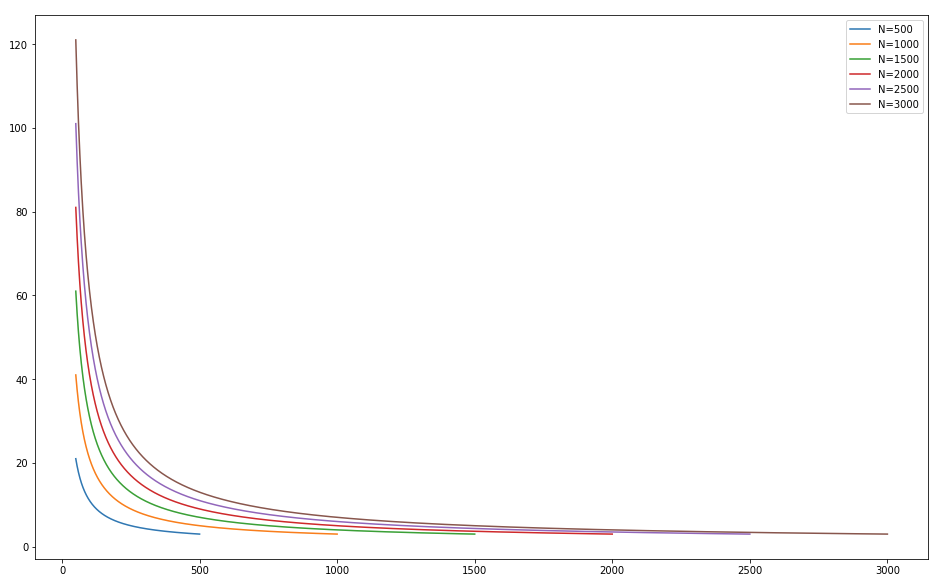
\includegraphics[width=\textwidth]{theory/img/B_times_diff_N}
	\caption{Графік залежності відношення $\frac{B_i^{n_1}}{B_i^{N}}$ від $n_1 \in [50, N]$ при фіксованих $N$ }
	\label{fig:one_diff_N}
\end{figure}

\section{Дискретна версія моделі обчислень множення матриць}
Нехай розмір блоку $n$ є дільником $N$, тоді задача множення матриць $N*N$ та $N*N$ поділяється на $k = \frac{N^2}{n^2}$ паралельних задач множення матриць $n*N$ та $N*n$.
У порівнянні з потоковою моделю, дискретний варіант має скінченну множину комбінацій розподілу задач планувальником на обчислювальні вузли.

Визначимо множину $Y(n)$ по аналогії з $X(n)$:

\begin{equation}
	\label{eq:Y(n)}
	Y(n) = \big\{y \in R^m : y_i \in {0, \ldots, k}, \sum_{j = 1}^{m} y_j = k, i = 1,\ldots,m \big\}
\end{equation}

Оскільки $Y(n)$ це дискретний варіант $X(n)$, то очевидне включення $Y(n) \subset X(n)$.
Задача планувальника є саме вибір конкретного вектора $y \in Y(n)$.
У роботі досліджуються планувальники типу $extr_1 extr_2$ - min min, min max, max min та max max. Принцип роботи їх дуже простий.

\begin{itemize}
	\item[1] Формується черга задач
	\item[2] Із черги задач вилучається задача згідно з конфігурацією $extr_1$. $min$ конфігурація вибирає задачу із черги з найменшою складністю, а $max$ з найбільшою
	\item[3] Вилучена з черги задача надсилається на вільний процесор згідно з правилом $extr2$. $min$ конфігурація має на меті виконати задачу за найкоротший час і вибирає вільний процесор з найбільшою потужністю, а $max$ навпаки - з найменшою
	\item[4] Якщо черга задач не пуста, то повернутися на крок 2
\end{itemize}

Твердження
Для будь-якого $n$ виконуються нерівності:
\begin{equation}
	T_d(n) = \min\limits_{y \in Y(n)} T(y, X(n))) \ge \min\limits_{x \in X(n)} T(x, X(n)))
\end{equation}

Також варто пояснити саму суть пошуку найкращого розбиття. Основна проблема у тому, що для великих розбиттів планування може бути недостаньо рівномірно розподелене. Наприклад, розглянемо систему з трьома однаковими обчислювальними вузлами. Розбиття матриць на 2 підматриці буде недостатньо ефективно оскільки будуть сформовані 4 задачі. 3 з 4 задач виконаються повністю паралельно, але четверта буде виконуватись на одному вузлі, в той час як інші 2 будут простоювати. Саме для цього ми і намагаємося розрізати матриці на рівні малі шматки, щоб такої проблеми не виникало. Проте через наявність штрафів за пересилку за затримок дуже малі розбиття також не підходять оскільки штрафи стають занадто великими.

Також з граничних випадків можна розгянути такий, при якому $q=\inf$ та $l=0$. Таку ситуацію можна зустріти при обчисленні добутку матриць на одному комп'ютері з кількома ядрами. Саме для цього випадку очевидно, що найкращою стратегією буде розрізати на найменші шматки. Таким чином буде мінімізований час простою при виконанні останніх задач з черги.

\section{Визначення з теорії ігор}

Нехай задана гра для $n$ осіб $(S,f)$, де $S$ - профіль стратегій $S=S_1 \times S_2 \times \ldots \times S_n$ та $f$ - функція виграшу $f=(f_1(x),f_2(x), \ldots, f_n(x))$ для $x \in S$.

Для деякого набору стратегій гравців $x \in S$ позначимо за $x_{-i}$ вектор $x$ без складової $i$, тобто стратегіями усіх гравців крім $i$-го.

Для $i$-го гравця кажуть, що $x^1_i$ домінує $x^2_i$, $x^1_i, x^2_i \in S_i$, якщо $f_i(x^1_i, x_{-i}) > f_i(x^2_i, x_{-i}), x_{-i} \in S_1 \times S_2 \times \ldots S_{i-1} \times S_{i+1} \times \ldots \times S_n$. Також кажуть, що $x^2_i$ домінована $x^1_i$. Також домінування може бути нестрогим, для цього у визначенні потрібно використовувати нестрогу нерівність.

\begin{table}[H]
	\centering
	\label{table:simple_game}
	\caption{Проста гра двох осіб у матричній формі}
	\begin{tabular}{|p{1cm}|p{1cm}|p{1cm}|p{1cm}|}
		\hline
		        & 1     & 2     & 3
		\\ \hline
		1 		& 1 , 2 & 2 , 2 & 3 , 5
		\\ \hline
		2 		& 2 , 1 & 3 , 4 & 4 , 3
		\\ \hline
		3 		& 3 , 5 & 3 , 7 & 5 , 8
		\\ \hline
	\end{tabular}
\end{table}

Простіше за визначення демонструвати для ігор двох гравців, оскільки їх можна представити у вигляді матриць \ref{table:simple_game}. У ній для першого гравця стратегія "2" домінує "1" та стратегія "3" нестрого домінує "2". Домінуючі стратегії допомагають при аналізі гри, оскільки фактично домінування одної стратегії "А" над "Б" дозволяє не розглядати стратегію "Б" у подальшому. У випадку раціональності гравця він ніколи не вибере доміновану стратегію.

Неформальне визначення рівноваги за Нешем звучить так: у точці рівноваги жоден з гравців не може збільшити свій виграш шляхом вибору іншої стратегії при фіксованих стратегіях інших гравців.

Запишемо формальне визначення рівноваги за Нешем.

$x^*$ є рівновагою за Нешем якщо:
\begin{equation}
	\forall i, x_i \in S_i : f_i(x^*_im x^*_{-i}) > f_i(x_i, x^*_{-i})	
	\label{eq:nash_equilibrium_def}
\end{equation}

Найпопулярнішою демонстрацією рівноваги за Нешем є дилема в'язня.

\begin{table}[H]
	\centering
	\label{table:prisoners_dillema}
	\caption{Ілюстрація дилеми в'язня як гри у матричній формі}
	\begin{tabular}{|l|l|l|}
		\hline
					& Співпраця & Зрада
		\\ \hline
		Співпраця 	& 2 , 2     & 10 , 1
		\\ \hline
		Зрада 		& 1 , 10    & 5 , 5
		\\ \hline
	\end{tabular}
\end{table}

Таблиця \ref{table:prisoners_dillema} показує типове визначення дилеми в'язня. У таблиці записані програші учасників, тобто кожен з них намагається мінімізувати свій програш і таким чином максимізувати виграш.

Пояснюється за ситуація тим, що двох в'язнів запитують про свідчення проти спільника. Якщо один в'язень надає свідчення про іншого, то йому трохи вкорочують строк перебування у в'язниці, а другому навпаки збільшують. Також якщо вони обидва будуть мовчати, то їм однаковий строк, який відносно виглядає оптимально порівняно з іншими. Проте якщо вони обидва будуть свідчити, то їм обом строк 5 років.

Як можна побачити з матриці, домінуючих стратегій немає. Проте є рівнована за Нешем. Рівновага у парі стратегій ("Зрада","Зрада"). Найцікавіше тут те, що точка рівноваги показує програші значно більші ніж у стратегії ("Співпраця","Співпраця"). Проте логіка при розгляданні рівноваги за Нешем полягає у пошуку найкращої відповіді на певну фіксовану стратегію опонента.

Ще одне неформальне визначення рівноваги за Нешем є "найкраща відповідь на найкращу відповідь".

Особливу увагу надають цій рівновазі саме через її застосування у теорії конфліктних ситуацій, оскільки саме точки рівноваги за Нешем часто описують ситуації, з яких важко вийти. Причому вихід з таких ситуацій не вигідний нікому, хоч і існують інші точки у грі, які можуть мати значно більші виграші.


\section{Некооперативна ігрова модель планування множення матриць для двох користувачів}

Сформулюємо концепції гри між двома гравцями, бажання яких є виконання задачі множення матриць у розподіленому середовищі з паралелізацією методом розбиття матриць на блоки. 

Некооперативна гра описує процес прийняття рішення про розбиття двома гравцями в умовах конфлікту інтересів. Некооперативність полягає у тому, що немає зовнішніх причин до їх співпраці, проте в самій грі з певною структурою може виникати співпраця гравців.

Нехай у загальному випадку ця гра проводиться між гравцями ${u_i}, i=1,\ldots,L$. Усі гравці мають рівний доступ до розподіленого середовища з потужностями обчислювальних вузлів ${p_i}, i=1,\ldots,m$ через спільний інтерфейс планувальника. Також передача даних для множення підблоків проходить по каналам з пропускними здатностями $q$ та затримкою $l$. Кожен з гравців може зареєструвати певний набір задач і після цього чекати на результат. Часом для гравця $u_i$ будемо вважати час повернення результата усіх відісланих ним задач, тобто момент, коли він отримає останній блок матриці результата.

Для гравців заданий розмір $N$ і їх задача порахувати у розподіленому середовищі добуток матриць $N*N$ та $N*N$. Стратегіями гравців називаемо $n_i \in [1,N]$ які визначають розмір блоку розбиття.

Кожен гравець хоче виконати паралельне множення матриць якможна швидше. Конфлікт полягає у тому, що зміна стратегії розбиття одним гравцем може покращити його час, проте значно погіршити час другого гравця.

Виділяють гравців раціональних та нераціональних. Дії раціонального гравця спрямовані на максимізацію його виграшу. Нераціональні можуть вносити хаос випадковими ходами. Вважатимемо, що гравці у цій грі раціональні.

Для спрощення будемо вважати, що виконуються такі припущення:
\begin{itemize}
	\item Страгерії користувачів $n_i, i=1,\ldots,k$ впорядковані за зростанням
	\item Стратегії користувачів $n_i$ є дільниками $N$
	\item У випадку, якщо користувачі вибрали однакове розбиття, то їх час завершення однаковий та дорівнює подвноєному індивідуальному часу
	\item Існує єдиний мінімум $T_d(n_j), j=1,\ldots,k$. Позначимо індекс, при якому досягається мінімум за $j^*$
\end{itemize}

Розглянемо планувальники min-min та min-max.

Нехай користувачі вибрали розрізання $n_1,n_2$, які являються їх стратегіями у грі. Користувачі відправляють свої задачі, та отримують результати. Часи повернення усіх задач позначимо за $T_1(n_1,n_2),T_2(n_1,n_2)$, які є власне програшами користувачів.

Враховуючи специфіку планувальників помітимо такі властивості часів повернення від розрізань:
\begin{itemize}
	\item Якщо $n_1 < n_2$, то виграш першого користувача дорівнює $T_d(n_1)$, а другого $T_d(n_1) + T_d(n_2)$
	\item Якщо $n_1 > n_2$, то виграш першого користувача дорівнює $T_d(n_1) + T_d(n_2)$, а другого $T_d(n_2)$
	\item Якщо $n_1 = n_2$, то виграші користувачів однакові та дорювнюють $2T_d(n_1)$
\end{itemize}

Такі властивості з'являються через те, що ці планувальники пріорітезують задачі з меншим обзягом роботи і тому користувач, який вибрав розрізання менше, повністю окупує обчислювальні ресурси. Задачі другого користувача підуть на виконання лише після того як усі задачі першого користувача будуть вилучені з черги очікування. Це явище і породжує конфлікт між двома гравцями, оскільки кожен з них хоче мінімізувати свій програш - час виконання власних задач. Пороте у минулих підрозділах ми розглянули форму штрафів для різних розбиттів і зменшувати розмір розбиття починаючи з деякого момента вносить дуже великий штраф за пересилання. Особливо це помітно у випадках коли ми розглядаємо розбиття $n: n \divides N$.

\textbf{Тверження}.

Нехай виконується нерівність
\begin{equation}
	2T_d(n_{j^*}) \le T_d(n_{{j^*}-1})
	\label{eq:le_min_both}
\end{equation}

тоді пара стратегій $(n_{j^*},n_{j^*})$ - рівновага Неша.

\textbf{Доведення}.

Розглянемо стратегію $(n_{j^*},n_{j^*})$ у випадку якщо нерівність \ref{eq:le_min_both} виконується, тоді отримуємо такі факти:
\begin{itemize}
	\item[1.] За властивостями планувальника якщо будь-який з користувачів змінить свою стратегію на $n: n > n_{j^*}$, тоді його програш тільки збільшиться, оскільки тоді перший користувач буде мати розмір розрізання менший і його виконані задачі в першу чергу.
	
	\item[2.] При зміні стратегії на $n_{j^*-1}$ користувач виграє право першочергового виконання саме його набору задач, проте завдяки нерівності \ref{eq:le_min_both} ця зміна стратегії не зменшить його програш.
	
	\item[3.] При зміні стратегії на $n: n < n_{j^* - 1}$ штрафні частини функції часу вже більше впливають на час і тому у реальних випадках ці стратегії дадуть значно більший штраф. Цей ефект краще всього буде проілюстровано у практичній частині в наведеній таблиці окремих компонент часу виконання в залежності від розбиття.
\end{itemize}

\textbf{Наслідок}.

Отримана рівновага Парето неефективна, оскільки $T_1(n_{j^*},n_{j^*}) < T_1(n_{j^*-1},n_{j^*-1})$ та $T_2(n_{j^*},n_{j^*}) < T_2(n_{j^*-1},n_{j^*-1})$.




 